%amsart class
\documentclass[a4paper, 10pt, reqno]{amsart}

%Packages
\usepackage[utf8]{inputenc}
\usepackage[english]{babel}
\usepackage{graphics}
%\usepackage{graphicx}
\usepackage{subcaption}
\usepackage{physics}
\usepackage{listings}
\usepackage{hyperref}
\usepackage{blindtext}
\usepackage{xcolor}
\usepackage{pgf}
\usepackage{pgfplots}
\usepackage{placeins}
\usepackage{parskip}


\hypersetup{colorlinks=true, linkcolor=black, citecolor=black, urlcolor=blue}
%\hypersetup{hidelinks}

\pgfplotsset{compat=1.5}
\newlength\figureheight
\newlength\figurewidth
\setlength\figurewidth{0.98\textwidth}
\setlength\figureheight{0.75\figurewidth}

\usepackage{etoolbox}
\makeatletter
\patchcmd{\@maketitle}
  {\ifx\@empty\@dedicatory}
  {\ifx\@empty\@date \else {\vskip3ex \centering\footnotesize\@date\par\vskip1ex}\fi
   \ifx\@empty\@dedicatory}
  {}{}
\patchcmd{\@adminfootnotes}
  {\ifx\@empty\@date\else \@footnotetext{\@setdate}\fi}
  {}{}{}
\makeatother

%Custom colors
\definecolor{code}{rgb}{0.9, 0.17, 0.31}
\definecolor{coolgrey}{rgb}{0.55, 0.57, 0.67}
\definecolor{cyan(process)}{rgb}{0.0, 0.72, 0.92}
\definecolor{lightwhite}{rgb}{0.9647058823529412, 0.9647058823529412, 0.9647058823529412}
\definecolor{royalblue}{rgb}{0.25, 0.41, 0.88}
\definecolor{mediumseagreen}{rgb}{0.24, 0.7, 0.44}
%listing customization
\lstset{ %
  backgroundcolor=\color{lightwhite},
  basicstyle=\ttfamily\footnotesize,        % the size of the fonts that are used for the code
  breakatwhitespace=true,         % sets if automatic breaks should only happen at whitespace
  breaklines=true,                 % sets automatic line breaking
  captionpos=b,                    % sets the caption-position to bottom
  commentstyle=\color{mediumseagreen},    % comment style
  deletekeywords={...},            % if you want to delete keywords from the given language
  escapeinside={\%*}{*)},          % if you want to add LaTeX within your code
  extendedchars=true,              % lets you use non-ASCII characters; for 8-bits encodings only, does not work with UTF-8
  frame=single,	                   % adds a frame around the code
  keepspaces=true,                 % keeps spaces in text, useful for keeping indentation of code (possibly needs columns=flexible)
  keywordstyle=\color{code},       % keyword style
  language=C++,                 % the language of the code
  otherkeywords={...},           % if you want to add more keywords to the set
  emph={int,char,double,float,unsigned,void,bool,RNG_int,agents,pow,fabs,RNG_real,C,Trade,arma,sort,DumpToFile },
  emphstyle={\color{royalblue}},
  rulecolor=\color{white},         % if not set, the frame-color may be changed on line-breaks within not-black text (e.g. comments (green here))
  numbers=left,
  showspaces=false,                % show spaces everywhere adding particular underscores; it overrides 'showstringspaces'
  showstringspaces=false,          % underline spaces within strings only
  showtabs=false,                  % show tabs within strings adding particular underscores
  stepnumber=1,                    % the step between two line-numbers. If it's 1, each line will be numbered
  tabsize=3,	                   % sets default tabsize to 2 spaces
}

%Frontpage stuff
\title[Compulsory Assignment 2]{\Large{Compulsory Assignment 2}\\
\normalsize{STK4900 - Statistical methods and applications}}

\author[Metin San]{Metin San}
\date{\today}



%Begining document
\begin{document}

\maketitle

\section{Introduction}
This is the second and final compulsory assignment in the course STK4900. It consists of three individual exercises. In the main part of the report, we will present and discuss the exercises along with the obtained results. The numerical code used to obtain the results  are attached in an appendix at the end of the report.


\section{Problem 1}
This exercise considers a study of horseshoe crabs on an island in the Gulf of Mexico. The purpose is to study how different features of the female horseshoe crab affects the number of present satellites (exterior male crabs which fertilized the females eggs during spawning). The variables considered in the study are
\begin{description}
    \item[y] Indicator for one or more satellites (0 $=$ no, 1 $=$ yes)
    \item[width] Width of carapace of female crab (in cm)
    \item[weight] Weight of female crab (in kg)
    \item[color] Color of female crab (1 $=$ medium light, 2 $=$ medium, 3 $=$ medium dark, 4 $=$ dark)
    \item[spine] Conditions of spine (1 $=$ both good, 2 $=$ one worn or broke, 3 $=$ both broken)
\end{description}

\subsection{a)}
We are interested in studying the effects of the covariate width, meaning that we must choose a suitable regression model.
Since we are working with binary data in that we are interested in $y =$ 0 or 1, a natural choice of model would be binary logistical regression. In general for a data set on the form $(x_1 , y_1), ... , (x_n, y_n$), where $y_i$ is a binary outcome (0 or 1) for subject $i$ and $x_i$ is a numerical or binary predictor (numerical in our case with width), the logistical regression model for a single covariate is given as
\begin{equation}
    p(x) = \frac{\exp(\beta_0 + \beta_1 x)}{1 + \exp(\beta_0 + \beta_1 x)}.
\end{equation}
Here, $p(x)$ is the probability, the $\beta_0$ and $\beta_1$ are the regression coefficients, and $x$ is the covariate of interest. This model results in a "S-shaped" relation between $p(x)$ and $x$.

Using this model in R produces the following fit summarized in table \ref{tab: 1}.

\begin{table}
\caption{Summary of the binary logical regression model for the predictor width.}
\label{tab: 1}
\begin{tabular}{lllllll}
\hline\hline
 & Estimate  & Std. Error & z value & Pr$(>\abs{\mathrm{z}})$ & \\ \hline
(Intercept) & -12.3508 & 2.6287   & -4.698  & 2.62e-06 & ***\\
width   & 0.4972 & 0.1017   & 4.887  & $<$ 1.02e-06 & ***\\
\hline
\end{tabular}
\end{table}

\subsection{b)}
We will now look to compute the odds ratio of presences of satellites between crabs that differ with 1 cm in width. The odds in a logistic model is given as
\begin{equation}
    \frac{p(x)}{1 - p(x)} = \exp(\beta_0 + \beta_1 x).
\end{equation}

The odds ratio, $OR$, between two subjects with covariate values $x$ and $x + \Delta$, are given as the ratio between their odds
\begin{equation}
    OR = \frac{\exp(\beta_0 + \beta_1(x + \Delta))}{\exp(\beta_0 + \beta_1 x)} = \exp(\beta_1 \Delta).
\end{equation}
In general, the odds ratio $\exp(\beta_1)$ corresponds to one unit increase in the covariate value. In our case, we want the odds ratio for a $\Delta = 1$ cm increase in width. This is then given as 
\begin{equation}
    \exp(\beta_1\Delta) = \exp(\beta_1) = \exp(0.4972) = 1.644,
\end{equation}
which corresponds to exactly one unit increase in width. This means that the odds of a female crab having satellites increases by $\approx 64\%$ if the width of the female increases by 1 cm.

The odds ratio can be approximated to the relative risk RR given as 

\begin{equation}
    RR = \frac{p(1)}{p(0)},
\end{equation}
if $p(1)$ and $p(0)$ are very small. For our fit, we find that for $x=1$, we get $p(1) = 7.12\times 10^{-6}$, and for $x = 0$ we get $p(0) = 4.33\times 10^{-6}$. These are very small numbers, suggesting that the approximation should hold. Computing the relative risk results in $RR = 1.644$, which shows that the approximation is very exact for our model. We can also find a 95 $\%$ confidence interval for the odds ratio through a script in R. Doing so results in the confidence interval $[1.346, 2.006]$.


\subsection{c)}
We proceed by performing the same analysis on the other covariates. The first two predictors width and weight are numerical covariates as they are continious. The third and forth covariates however in color and spine are discrete covariates as they can only take on finite values. This means that they are categorical variables, and we need to include these as factors in R. The purpose of the spine covariate it to check whether both spines are functioning or if both are broken, or if just one of them are working. It is therefore natural for it to be categorical as it only takes on 3 definite values. The color variable is hard to quantify as color is really a continuous spectrum. It has therefore been categorized into 4 groups which simplifies the observational aspect. The covariate could also have been a numerical predictor normalized to for instance the brightest and darkest crabs observed. Grouping covariates can sometimes result in models with better fit. This can be tested through a deviance test. 

Performing the same analysis for all covariates seperatly leaves us with the following models seen in table \ref{tab: 2}. 

\begin{table}
\caption{Summary of the binary logical regression models for each covariate separately.}
\label{tab: 2}
\begin{tabular}{llllllll}
\hline\hline
Model & & Estimate  & Std. Error & z value & Pr$(>\abs{\mathrm{z}})$ & \\ \hline

\textbf{Width}&(Intercept) & -12.3508 & 2.6287   & -4.698  & 2.62e-06 & ***\\
&width   & 0.4972 & 0.1017   & 4.887  & $<$ 1.02e-06 & ***\\
\hline

\textbf{Weight} &(Intercept) & -3.6947 & 0.8802   & -4.198  & 2.70e-05 & ***\\
&weight   & 1.8151 & 0.3767   & 4.819  & $<$ 1.45e-06 & ***\\ \hline

\textbf{Color}    &    (Intercept)    &  1.0986  &   0.6667   &1.648 &  0.0994 &.\\
&factor(color)2 & -0.1226 &    0.7053 & -0.174 &  0.8620  &\\
&factor(color)3 & -0.7309 &    0.7338 & -0.996  & 0.3192  &\\
&factor(color)4  &-1.8608  &   0.8087&  -2.301 &  0.0214 &*\\ \hline

\textbf{Spine}& (Intercept)   &   0.8602  &   0.3597 & 2.392  & 0.0168 &* \\
&factor(spine)2 & -0.9937  &   0.6303 & -1.577&   0.1149  &\\
&factor(spine)3 & -0.2647  &   0.4068 & -0.651 &  0.5152 &\\
\hline
\end{tabular}
\end{table}

From table \ref{tab: 2} we observe that the models for width and weight appear to both be highly significant on the presence of satellites. The categorical covariates color and spine seem to have much less of a significance. The spine model has high p values for all factors. The same is true for color with the exception of the factor(color)4, which corresponds to a dark color, which has some significance.

It should be noted that the apparent categorical estimates are normalized to their respective factor(..)1 values, which is why we only have 3 colors and 2 spine estimates.

\subsection{d)}
We will now fit a multiple logistic regression model where we use all covariates instead of each of them one by one. The resulting model can be seen in table \ref{tab: 3}.


\begin{table}
\caption{Summary of the multi binary logical regression model, using all covariates.}
\label{tab: 3}
\begin{tabular}{lllllll}
\hline\hline
 & Estimate  & Std. Error & z value & Pr$(>\abs{\mathrm{z}})$ & \\ \hline
(Intercept)  &  -8.06501 &   3.92855 & -2.053  & 0.0401& *\\
width&           0.26313&    0.19530&   1.347&   0.1779&  \\
weight   &       0.82578  &  0.70383 &  1.173  & 0.2407 & \\
factor(color)2& -0.10290  &  0.78259 & -0.131 &  0.8954 & \\
factor(color)3& -0.48886  &  0.85312&  -0.573  & 0.5666 & \\
factor(color)4& -1.60867  &  0.93553&  -1.720  & 0.0855 &.\\
factor(spine)2& -0.09598  &  0.70337 & -0.136  & 0.8915 & \\
factor(spine)3 & 0.40029   & 0.50270 &  0.796  & 0.4259 & \\
\hline
\end{tabular}
\end{table}

From table \ref{tab: 3} we see that such a model which includes all covariates results in non of the covariates being significant anymore. This is perhaps a result of overfitting as we include covariates which we know to mostly be non-significant. We therefore make another model using multiple logistic regression, but this time we only include the two covariates width and weight which were the dominating significant covariates. Doing so results in the following model summarized in table \ref{tab: 4}

\begin{table}
\caption{Summary of the multi binary logical regression model, using only the most significant covariates width and weight.}
\label{tab: 4}
\begin{tabular}{lllllll}
\hline\hline
 & Estimate  & Std. Error & z value & Pr$(>\abs{\mathrm{z}})$ & \\ \hline
(Intercept) & -9.3547    & 3.5280 & -2.652 & 0.00801& **\\
width   &      0.3068   &  0.1819  & 1.686 & 0.09177 &. \\
weight   &     0.8338   &  0.6716&   1.241 & 0.21445  & \\
\hline
\end{tabular}
\end{table}

We observe that the new model results in neither the width or weight being very significant. In order to investigate why the high significance levels in the two covariates width and weight are lost when combined, we need to look at the relation between the two covariates. We start by plotting the width of the female horseshoe crabs as a function of their respective weight. The results are seen in figure \ref{fig: corr}.

\begin{figure}
    \centering
    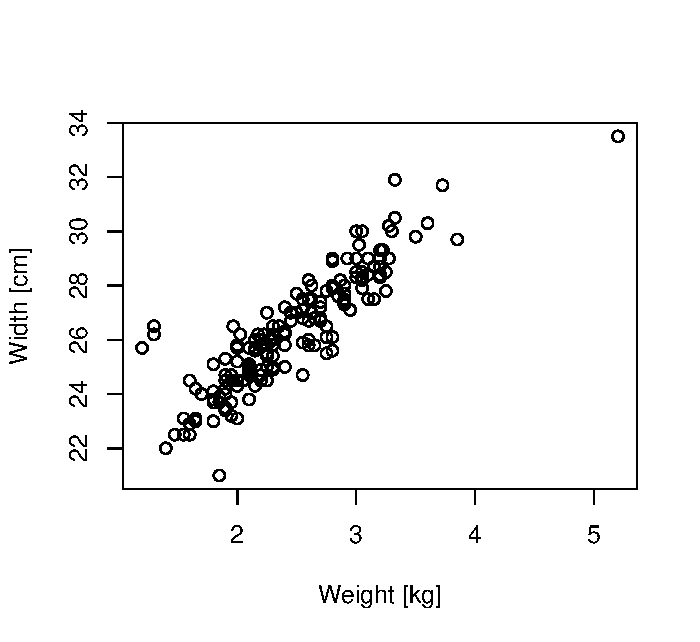
\includegraphics[width = 0.8\textwidth]{corr.pdf}
    \caption{Width of female horseshoe crabs as a function of their weight.}
    \label{fig: corr}
\end{figure}

From figure \ref{fig: corr} we immediately see a strong linear correlation between the two covariates. A heavier crab means a wider crab, as one one would excpect. The pearson correlation coefficient between the two predictors are 0.887 meaning that the correlation is highly linear. 

We can therefore say that the covariate width is the confounder for weight, meaning that we only really need to include one of these variables in our model. The final model is then constructed using either the width or weight, we have chosen width, as it might be the "visual" covariate out of the two which the horseshoe crabs might base their decisions of. The model is summarized in table \ref{tab: final}, in which we see that the significance of the covariate is back.

\begin{table}
\caption{Coefficients of the final model using only width as a covariate as summarized by R.}
\label{tab: final}
\begin{tabular}{lllllll}
\hline\hline
 & Estimate  & Std. Error & z value & Pr$(>\abs{\mathrm{z}})$ & \\ \hline
(Intercept)& -12.3508  &   2.6287&  -4.698& 2.62e-06& ***\\
width     &    0.4972  &   0.1017 &  4.887 &1.02e-06& ***\\
\hline
\end{tabular}
\end{table}

\subsection{e)}
It can also be of use to check whether or not our covariates have any interactions between them. That is when two binary predictors have causal effect on the outcome. We know that weight and width are confounding covariates. By fitting a model which includes interactions for the pair combination of spine and color with width, we find that there are in fact no significant interactions between the covariates in this study.

\section{Problem 2}
In this exercise we will analyze and study data from the 1996 and 2000 Olympics games. The goal is to see weather or not participants from larger and wealthier nations are more likely to win medals. The data we will be using considers 66 nations that won at least one medal during these games. The variables we will look at during our study are

\begin{description}
    \item[Total2000] Number of medals won by the nation in the Olympics of 2000
    \item[Total1996] Number of medals won by the nation in the Olympics of 1996
    \item[Log.population] Logarithm of the nation's population size per 1000
    \item[Log.athletes] Logarithm of the number of athletes representing the nation
    \item[GDP.per.cap] The per capita Gross Domestic Product of nation
\end{description}

\subsection{a)}
In order to start analyzing the data we need to pick a model. The outcome of the study is the number of medals earned by a nation, which makes it a count outcome. A natural model to use when working with count variables are Possion regression. We will therefore say that the count is distributed as $Y \sim $ Po$(\lambda)$, where the parameter $\lambda$ is the rate. We are working with a multicovariate model, meaning that the parameter $\lambda$ is not necessarily the same for all subjects. Our model then becomes $Y_i \sim$ Po$(\lambda_i)$ with a rate on the form
\begin{equation}
    \lambda_i = \lambda(x_{1i},x_{2i},...,x_{pi}) = \exp(\beta_0 + \beta_1 x_{1i} + \beta_2 x_{2i} + ... + \beta_p x_{pi}).
\end{equation}
If one works with aggregated counts, an observation $y_i$ is a realization of $Y_i \sim $Po$(w_i\lambda_i)$ where the weight $w_i$ is the number of subjects in group $i$. This is important for us as countries with a higher number of athletes have a higher probability of winning a medal, meaning that we need to include such a weight.

The expectation of the count is then given as 
\begin{align}
    E(Y_i) = w_i \lambda_i = & w_i \exp(\beta_0 + \beta_1 x_{1i} +\beta_2 x_{2i} + ... + \beta_p x_{pi})\\
    = & \exp(\log(w_i) +\beta_0 + \beta_1 x_{1i} +\beta_2 x_{2i} + ... + \beta_p x_{pi}),
\end{align}
where the term $\log(w_i)$ is a "covariate" where the regression coefficient is equal to 1. This term is also called the offset, and adding such a term to our model will compensate for the athlete number imbalance. A natural choice for such a covariate would be the Log.atheletes which we already have in our data.

\subsection{b)}
We will now attempt to find a best fit model to the provided data. We start by fitting a Possion regression with the covariates Total1996, Log.population and GDP.per.cap with Log.athletes as the offsett. This results in the following model seen in table \ref{tab: 5}

From the first model in table \ref{tab: 5}, we see that the most significant covariate is Total1996, followed by GDP.per.cap. The fact that the results of the previous Olympics appears to be the most important factor comes as no big surprise. Many of the previous contenders which won are likely to compete again and the existing infrastructure around the the Olympic games which have proven to work are likely still in place.

The correlation between Total1996 and Total2000 is 0.967, which means that the above model is highly multicollinear. This can cause problems when trying to interperet the results. In addition, using the previous years medal winners as the dominating covariate is comparable to a weather forecast basing their results on yesterdays weather. They will likely be correct to some degree, but we learn nothing of statistical importance. 

\begin{table}
\caption{Summary of the Possion regression model, using all covariates with Log.athletes as the offset.}
\label{tab: 5}
\begin{tabular}{lllllll}
\hline\hline
 & Estimate  & Std. Error & z value & Pr$(>\abs{\mathrm{z}})$ & \\ \hline
(Intercept)  &  -2.862299 &  0.319076 & -8.971 & < 2e-16& ***\\
Total1996      & 0.011832 &  0.001607 &  7.364& 1.79e-13 &***\\
Log.population & 0.027510 &  0.031539   &0.872 &   0.383 &   \\
GDP.per.cap   & -0.014924 &  0.003208 & -4.652& 3.29e-06 &***\\
\hline
\end{tabular}
\end{table}

\begin{table}
\caption{Summary of the Possion regression model, using a model without the covariate Total1996.}
\label{tab: 6}
\begin{tabular}{lllllll}
\hline\hline
 & Estimate  & Std. Error & z value & Pr$(>\abs{\mathrm{z}})$ & \\ \hline
(Intercept)  &  -4.255144  & 0.250782& -16.968 & < 2e-16 ***\\
Log.population & 0.179605 &  0.022466  & 7.995 & 1.3e-15 ***\\
GDP.per.cap  &  -0.004340&   0.002726 & -1.592  &  0.111  \\
\hline
\end{tabular}
\end{table}

We will therefore try a model without Total1996 to see what the significance of the other covariates are in this case. From table \ref{tab: 6} we see that this time around the Log.population is the most significant covariate, while GDP.per.cap is no longer any significant. By removing the insignificant GDP.per.cap, we end up with the final model seen in table \ref{tab: 7}

\begin{table}
\caption{Summary of the Possion regression model, using only Log.population as covariate.}
\label{tab: 7}
\begin{tabular}{lllllll}
\hline\hline
 & Estimate  & Std. Error & z value & Pr$(>\abs{\mathrm{z}})$ & \\ \hline
(Intercept) &   -4.34619  &  0.24585& -17.678 & < 2e-16 ***\\
Log.population & 0.18212 &   0.02256  & 8.073 &6.84e-16 ***\\
\hline
\end{tabular}
\end{table}

We can compute the rate ratio, $RR$, for this model, which is given as 
\begin{equation}
    RR = \exp(\beta_j) = \exp(0.182) = 1.997,
\end{equation}
which means that the rate of medals won by a nation increases by $\approx 20\%$ for one unit increase in Log.population. 


Our findings tell us that if we are interested in predicting which nations will win medals in the next Olympics, the best source would be to check the last years winners. However, if one are interested in checking out the winners of an arbritary Olympics, without the knowledge of the previous winners, the best bet would be to look at he population of the nation. We do however see in the data that countries such as India which has one of the highest Log.pop values only won 1 medal in both 2000 and 1996. This means that the model only considering the population can be very wrong for some scenarios. There are likely some covariates which are also significant such as the public information and the levels of education in a nation.

To conclude, it seems that the wealth of the country does not matter much when it comes to their medal count. Large countries however are more likely to bring home more medals.

\section{Problem 3}
We will now consider a study done on 488 patients with liver cirrhosis at various hospitals in Copenhagen. The purpose of the study was to investigate whether patients that was treated with the hormone prednisone had better survival than patients who got a placebo treatment. The variables available to us in the study are

\begin{description}
    \item[status] Indicator for death/censoring (1=dead, 0=censored)
    \item[time] Time in days from start of treatment to death/censoring
    \item[treat] Treatment (0=prednisone, 1=placebo)
    \item[sex] Gender (0=female, 1=male)
    \item[asc] Ascites at start of treament (0=none, 1=slight, 2=marked)
    \item[age] Age in years at start of treatmen
    \item[agegr] Age group (1=$<$50, 2=50-65, 3=$>$65)
\end{description}

\subsection{a)}
We start by looking at the survival of the studied patients. We will do so by making Kaplan-Meier plots for the following covariates: treat (prednisone or placebo), sex (female or male), asc (the severity of built up abdomen fluid) and agegr (age group). The results can be seen in figure \ref{fig: 1}. 

From figure \ref{fig: 1a} which shows the treatment survival function. We observe that the patients with the prednisone treatment have slightly lower survival during the first 1000 days compared to those with the placebo treatment. For most of the remaining time however, the prednisone treatment seem to increase the survival of the patients.

Figure \ref{fig: 1b} shows the survival function between the two genders. We observe a marginal difference, where the females patients have a higher survival compared to their male counterparts.

In figure \ref{fig: 1c} we see the survival function of the patients which started out with different levels of ascites. We observe that the patients with no ascites have the highest survival while those with the most ascites have the lowest.

From figure \ref{fig: 1d} which shows the survival function of the different age groups we observe that higher age means a lower survival, while a lower age results in a higher survival.

\begin{figure}
\makebox[\textwidth][c]{
  \begin{subfigure}[t]{0.7\textwidth}
    \centering
    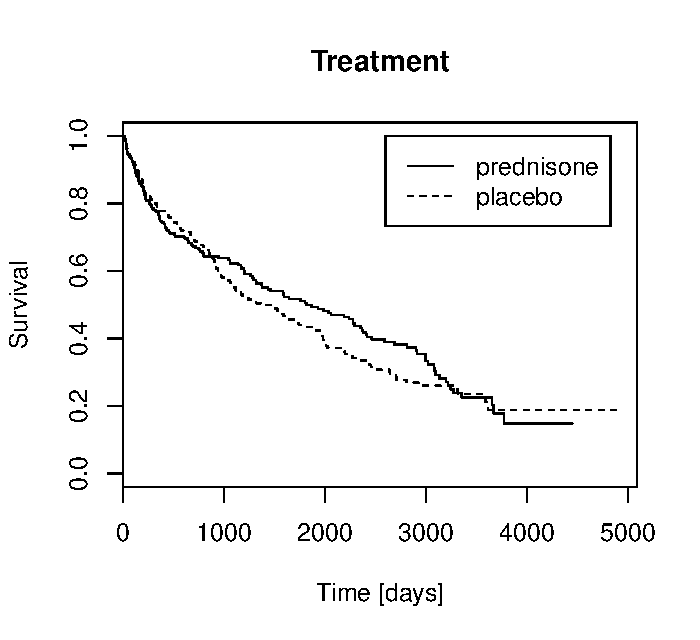
\includegraphics[width=0.9\textwidth]{treat.pdf} 
    \caption{Survival function for the two treatements.} 
    \label{fig: 1a} 
  \end{subfigure}%% 
  \begin{subfigure}[t]{0.7\textwidth}
    \centering
    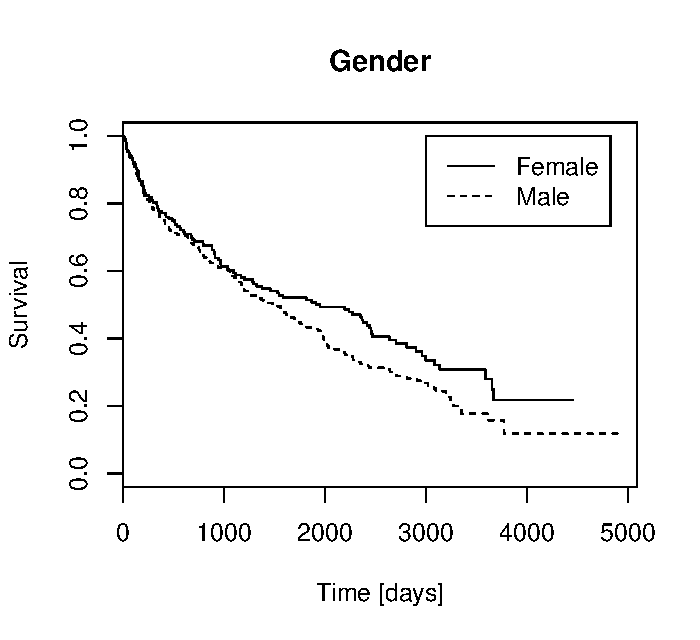
\includegraphics[width=0.9\textwidth]{sex.pdf}
    \caption{Survival function for the genders.} 
    \label{fig: 1b} 
  \end{subfigure} 
  }
  \makebox[\textwidth][c]{
  \begin{subfigure}[t]{0.7\textwidth}
    \centering
    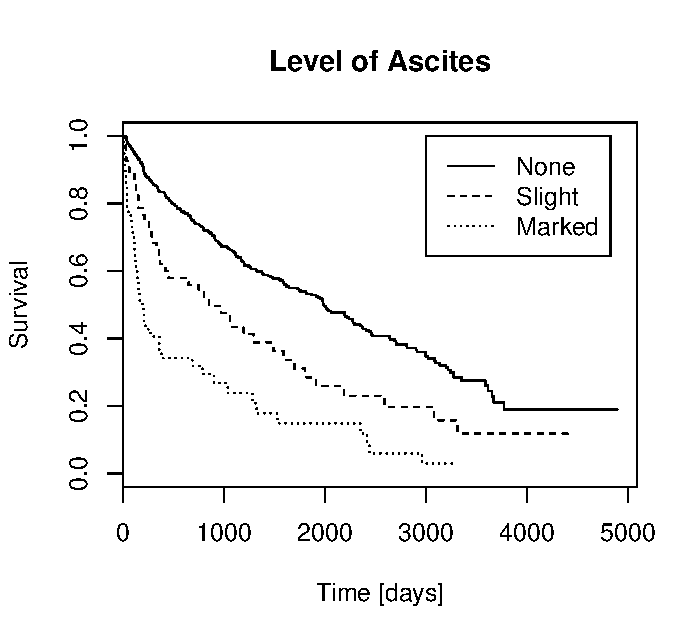
\includegraphics[width=0.9\textwidth]{asc.pdf}
    \caption{Survival function for the initial level of ascites in the patients.} 
    \label{fig: 1c} 
  \end{subfigure}%%
  \begin{subfigure}[t]{0.7\textwidth}
    \centering
    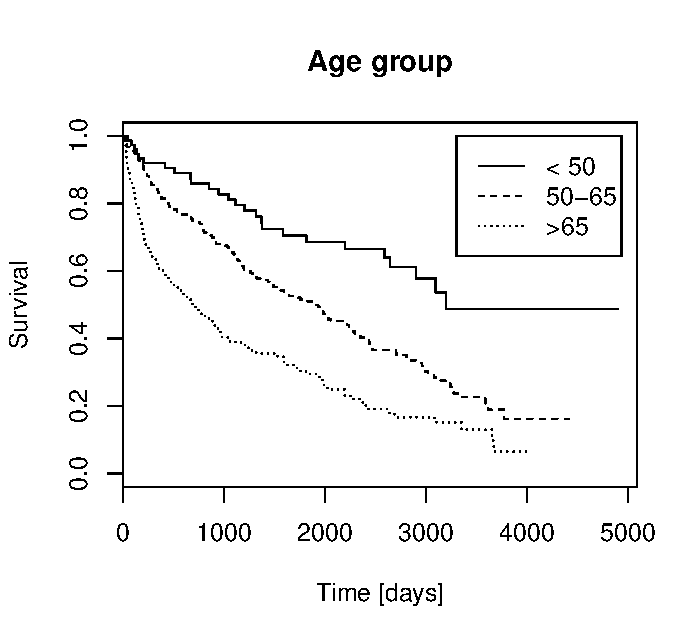
\includegraphics[width=0.9\textwidth]{agegr.pdf}
    \caption{Survival function for the different age groups.} 
    \label{fig: 1d} 
  \end{subfigure} 
  }
  \caption{Survival functions for the four covariates of interest: treat, sex, asc and agegr.}
  \label{fig: 1} 
\end{figure}

\subsection{b)}
From the Kaplan-Meier plots we observed differences in the different groups. We will now check if these differences are significant through the use of logrank tests, which is a way of testing the null hypothesis. Our null hypothesis will be that the survival function is the same in both treatment groups so that 
\begin{equation}
    H_0: S_1(t) = S_2(t), \quad  \forall \quad t.
\end{equation}

We will use the test statistic $\chi^2$ which is given as
\begin{equation}
    \chi^{2}_i=\frac{\left(O_{i}-E_{i}\right)^{2}}{\widehat{\operatorname{se}}\left(O_{i}-E_{i}\right)^{2}}.
\end{equation}
Here $O_i$ is the observed number of events and $E_i$ is the expected number of events in group $i$. 

Performing the above test gives us the results seen in table \ref{tab: treat} through \ref{tab: agegr}. Even though the survival function for the prednisone treated group seems like it does increase the survival from the plots, the logrank test in table \ref{tab: treat} results in $\chi^2 = 0.7$ which is fairly low and a p-value of $p=0.4$. This means that we should not draw conclusions about the increased survival of the treated group just yet. 

The gender dependence in in figure \ref{fig: 1b} does seem significant, however, from the logrank test from \ref{tab: sex} we get a $\chi^2 = 3.5$ and $p = 0.06$. These values are not significant enough to be able to reject the null hypothesis, meaning that we again can not conclude that there are differences in survival between males and females. 

In the case of the asc and agegr survival functions it is visually clear that the null hypothesis in both cases are wrong. This is strongly confirmed by the log rank tests in tables \ref{tab: asc} and \ref{tab: agegr} which result in huge $\chi^2$ values and very small p-values.


\begin{table}
\caption{}
\label{tab: treat}
\begin{tabular}{lllllll}
\hline\hline
 & N  & Observed & Expected &$(O-E)^2/E$ & $(O-E)^2/V$\\ \hline
treat=0 &251  &    142   &   149 &    0.355  &   0.728\\
treat=1 &237   &   150    &  143 &    0.371  &   0.728\\
\multicolumn{4}{l}{Chisq= 0.7  on 1 degrees of freedom, p= 0.4 }\\
\hline

\end{tabular}
\end{table}
\begin{table}
\caption{}
\label{tab: sex}
\begin{tabular}{lllllll}
\hline\hline
 & N  & Observed & Expected &$(O-E)^2/E$ & $(O-E)^2/V$\\ \hline
sex=0 &198  &    111   &   127   &   2.00  &    3.55\\
sex=1 &290  &    181   &   165   &   1.54   &   3.55\\
\multicolumn{4}{l}{Chisq= 3.5  on 1 degrees of freedom, p= 0.06 }\\
\hline

\end{tabular}
\end{table}

\begin{table}
\caption{}
\label{tab: asc}
\begin{tabular}{lllllll}
\hline\hline
 & N  & Observed & Expected &$(O-E)^2/E$ & $(O-E)^2/V$\\ \hline
asc=0& 386    &  211   & 251.9   &   6.63  &   48.66\\
asc=1 & 54    &   39   &  26.2   &   6.30  &    6.94\\
asc=2&  48    &   42    & 14.0   &  56.17  &   59.60\\
\multicolumn{4}{l}{Chisq= 69.9  on 2 degrees of freedom, p= 7e-16}\\
\hline

\end{tabular}
\end{table}

\begin{table}
\caption{}
\label{tab: agegr}
\begin{tabular}{lllllll}
\hline\hline
 & N  & Observed & Expected &$(O-E)^2/E$ & $(O-E)^2/V$\\ \hline
agegr=1&  80     &  26  &   58.7   &  18.18   &  22.87\\
agegr=2 &250    &  148   & 162.0   &   1.21   &   2.72\\
agegr=3& 158    &  118   &  71.3   & 30.51   &  40.87\\
\multicolumn{4}{l}{Chisq= 50.6  on 2 degrees of freedom, p= 1e-11 }\\
\hline

\end{tabular}
\end{table}


\subsection{c)}

Another way to study survival data is through so called proportional hazard models. In general, a multicovariate hazard function is given as
\begin{equation}
    h\left(t | x_{1}, x_{2}, \ldots, x_{p}\right)=h_{0}(t) \exp \left(\beta_{1} x_{1}+\beta_{2} x_{2}+\ldots .+\beta_{p} x_{p}\right),
\end{equation}
where $h_0(t)$ is the baseline hazard for a subject with all covariates equal to zero. We will now estimate the hazard function through a multiple Cox regression where we will study all the covariates simultaneously. Doing so with the use of R results in the following model seen in table \ref{tab: cox}

\begin{table}
\caption{Summary of the Cox regression.}
\label{tab: cox}
\begin{tabular}{lllllll}
\hline\hline
            &       coef& exp(coef)& se(coef) &    z &Pr$(>|z|)$ & \\ \hline  
factor(sex)1 &  0.461877 & 1.587050& 0.125631& 3.676& 0.000236 &***\\
factor(treat)1 &0.044818  &1.045837 &0.117657 &0.381 &0.703263 &   \\
factor(asc)1 &  0.603507&  1.828520& 0.175019& 3.448 &0.000564 &***\\
factor(asc)2  & 1.187254 & 3.278068 &0.175224& 6.776& 1.24e-11 &***\\
age      &      0.048877 & 1.050091 &0.006844 &7.141 &9.26e-13 &***\\
\hline
\end{tabular}
\end{table}
From table \ref{tab: cox} we again see that age and asc are both highly significant covariants. In contrast to the logrank test however, sex is now also a significant covariant with a p-value of $p=0.0002$.

We can also find the hazard ratio, HR, which is given as
\begin{equation}
    HR = \frac{h\left(t | x_{1}+\Delta, x_{2}, \ldots, x_{p}\right)}{h\left(t | x_{1}, x_{2}, \ldots, x_{p}\right)}=\exp \left(\beta_{1} \Delta\right),
\end{equation}
where $\exp(\beta_1)$ is the hazard ratio corresponding to one units increase in the value of the covariate $x_1$ while all other covariates are held condstant. For our model, if we consider the hazard ratio for males and females, we find

\begin{equation}
    \exp \left(\beta_{\text {sex}}\right)=\exp (0.461)=1.587,
\end{equation}
meaning that the hazard increases by a whole $\approx 58.7\%$ if the subject is male. 

We can also find the $95\%$ confidence interval for the above ratio from the usual $\exp \left(\beta_{i}\right) \pm \exp \left(1.96 \cdot \operatorname{se}\left(\beta_{i}\right)\right)$. From R, we find the confidence interval to be $[1.24, 2.03]$ for the sex hazard ratio. Since 1 is not in the confidence interval, we can conclude that the hazard is significant.

We see the importance of using multiple models to analyze the survival data, as the logrank method and Cox regression yield different results on the significance of the sex covariant. We can however not conclude that the effects of the prednisone treatment has any significant benefits on the survival of the patients tested.
\section{Appendix}
Here follows the code for exercise 1,2 and 3

\subsection{Exercise 1}

\lstinputlisting[language=R, firstline=1, lastline=63, caption={} , label=lst: equilibrium]{problem1.R}

\subsection{Exercise 2}

\lstinputlisting[language=R, firstline=1, lastline=31, caption={} , label=lst: equilibrium]{problem2.R}

\subsection{Exercise 3}

\lstinputlisting[language=R, firstline=1, lastline=31, caption={} , label=lst: equilibrium]{problem3.R}

\nocite{*}
\bibliography{references}{}
\bibliographystyle{plain}
\end{document}

